\documentclass[a4paper, 11pt]{article}

\usepackage{xcolor}
\input{/home/aroquemaurel/cours/includesLaTeX/couleurs.tex}
\usepackage{lmodern}
\usepackage[utf8]{inputenc}
\usepackage[T1]{fontenc}
\usepackage[francais]{babel}
\usepackage[top=1.7cm, bottom=1.7cm, left=2.5cm, right=2.5cm]{geometry}
\usepackage{verbatim}
\usepackage{tikz} %Vectoriel
\usepackage{pgfplots}
\usepackage{listings}
\usepackage{fancyhdr}
\usepackage{multido}
\usepackage{amssymb}
\usepackage{multicol}
\usepackage{float}
\usepackage[urlbordercolor={1 1 1}, linkbordercolor={1 1 1}, linkcolor=vert1, urlcolor=bleu, colorlinks=true]{hyperref}

\newcommand{\titre}{Compression d'image en niveaux de gris}
\newcommand{\numero}{1}
\newcommand{\typeDoc}{DM}
\newcommand{\module}{Outils Informatiques pour le Multimédia}
\newcommand{\sigle}{OIM}
\newcommand{\semestre}{7}

\input{/home/aroquemaurel/cours/includesLaTeX/l3/tddm.tex}
\input{/home/aroquemaurel/cours/includesLaTeX/listings.tex} %prise en charge du langage C 
\input{/home/aroquemaurel/cours/includesLaTeX/l3/remarquesExempleAttention.tex}
\input{/home/aroquemaurel/cours/includesLaTeX/polices.tex}
\input{/home/aroquemaurel/cours/includesLaTeX/affichageChapitre.tex}
\makeatother
\begin{document}
	\maketitle
	\section{Compilation exécution et tests}
	L'archive qui à été déposée sur Moodle est organisé comme suit : 
	\begin{description}
		\item[\texttt{Report\_deRoquemaurelAntoine\_G1.1.pdf}] Le rapport que vous êtes en train de consulter
		\item[\texttt{Compressor/}] Programme de compression contenant les fichiers détaillés section \ref{files}. 
	\end{description}
	\subsection{Fichier sources}	
	\begin{itemize}
		\item \texttt{block.c} : Fonctions et structures de données concernant les blocks.
		\item \texttt{compressor.c} : Fonctions de compression.
		\item \texttt{decompressor.c} : Fonctions de décompression.
		\item \texttt{main.c} : Fichier principal gérant les arguments
		\item \texttt{ZIterator.c} : Itérateur effectuant un parcours en Z.
		\item \texttt{blockiterator.c} : Itérateur permettant de parcourir une image block par block.
		\item \texttt{dct-idct.c} : Fonctions appliquant la dct et son inverse
		\item \texttt{image.c} : Fonctions et structure de données concernant les images
		\item \texttt{util.c} : Fonctions utiles
		\item \texttt{Makefile} : Fichier Makefile
	\end{itemize}

	\subsection{Fichiers de tests}
	L'exécution des tests s'effectue de la même manière que l'archive fournie : 
	\begin{lstlisting}[language=Bash, caption=Execution des tests, label=lst:test]
aroquemaurel@aokiji < master > : ~/projets/c/oim/jpg-compression/report
[0] % time make tests 
dct           [OK]
quantify      [OK]
vectorize     [OK]
compression   [OK]
decompression [OK]
make tests  0,38s user 0,07s system 85% cpu 0,532 total
	\end{lstlisting}
	\label{files}

	Comme montré listing \ref{lst:test}, l'intégralité des tests passent, ceux-ci sont basés sur les images d'origine. Un image de taille plus importante à été
	ajoutée afin de pouvoir mieux observer les différentes optimisation, plus d'informations sont fournies section \ref{opti}.

	\section{Compression}
	Afin d'effectuer la compression, plusieurs tests ont été effectués afin de garantir que chaque module était bien fonctionnel : 
	\begin{itemize}
		\item Dct
		\item Quantify
		\item Vectorize
		\item Compression
	\end{itemize}

	Chaque test est incrémental : un test ne peut pas passer sans passer le précédent.

	\subsection{Dct et Quantify}
	Afin d'appliquer la dct et de quantifier la matrice, il faut utiliser la fonction \texttt{applyDct} qui en fonction du 3\ieme{} paramètre applique soit la
	normalisation, c'est-à-dire une division par \texttt{8.f}, soit il divise par la matrice de quantification. Cette factorisation nous permet de réutiliser
	cette méthode soit pour le test dct, soit pour le test quantify. 

	\subsection{Vectorize}
	La vectorisation consiste en l'utilisation d'un Itérateur permettant de parcourir un block en Z comme le montre l'image ci-contre.

	Cet itérateur, \texttt{ZIterateur}, possède les méthodes \texttt{has\_next} et \texttt{next} permettant de parcourir l'intégralité du block comme le montre
	le listing \ref{lst:zit}. La méthode
	\texttt{next} doit vérifier tous les cas possibles avant de renvoyer la bonne valeur et de déplacer le curseur dans le tableau. 
	\begin{lstlisting}[language=C, caption=Vectoriser une image, label=lst:zit]
	for(i = 0 ; i < input->h ; i +=8 ) {
		for(j = 0 ; j < input->w ; j += 8) {
			block = block_new();
			dct(input, block.data, j, i);
			block_applyQuantify(&block, quantify);
			zit = zIterator_new(block, 8);

			output->data[(output->size)++] = round(zIterator_value(zit)); 
			while(zIterator_hasNext(zit)) {
				output->data[(output->size)++] = round(zIterator_next(&zit));
			}

			zIterator_delete(&zit);
			block_delete(&block);
		}
	}
			\end{lstlisting}	
	Une solution plus optimisée que la présente aurait pu être de générer la liste des positions nécessaires à un déplacement en Z avec un script externe tel que
	Python ou Bash. Cependant cette solution était moins souple en terme d'évolution : l'execution 

	Une autre solution peut cependant être envisager pour optimiser un peu plus l'algorithme : stocker les valeurs des cases devant être parcourues dans un
	tableau.

	\section{Décompression}
	La décompression utilise globalement les modules déjà développés précédemment, cependant en raison de l'\texttt{idct} particulièrement lente, une étape d'optimisation
	section \ref{opti} sera nécessaire.

	Figure \ref{fig:mystere}, nous pouvons voir l'image \texttt{mystery.xxx} une fois décompressée grâce au développement du décompresseur.

\begin{attention}
	La décompression fonctionne correctement sur les systèmes 64bits, il semblerait cependant que le test de décompression renvoit \texttt{KO} sur un système
	32bits. 

	Cela vient d'une approximation des arrondies, bien que l'image reste tout à fait lisible. On peut supposer que la compression / décompression sous un système
	32 bits à un taux d'erreur plus important.

	Il est conseillé de tester le compresseur sur un système 64bits.
\end{attention}
	\begin{figure}[H]
		\centering
		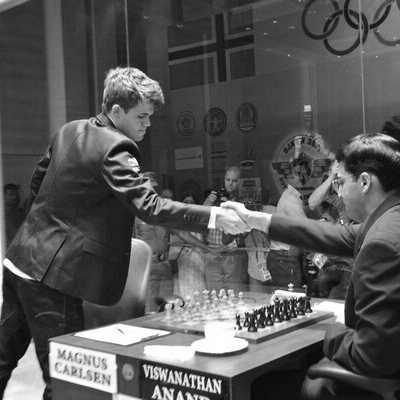
\includegraphics[width=8cm]{mystery.jpg}
		\caption{Image mystère}
		\label{fig:mystere}
	\end{figure}

	\section{Optimisations}\label{opti}
	Le traitement d'image, et particulièrement la décompression sont des opérations couteuses. Ainsi afin d'avoir un traitement qui soit correct en mémoire
	ou en cpu, des optimisations étaient nécessaires. 

	Deux axes d'optimisations ont été travaillés : 
	\begin{itemize}
		\item D'une part, limiter les calculs, notamment dans les boucles, et particulièrement pour la fonction idct. 
		\item D'autres part, l'utilisation de plusieurs cœurs en parallélisant le système semblait être intéressant.
	\end{itemize}
	
	Afin de pouvoir observer facilement le temps d'exécution gagné, une image à été ajouté aux scripts de tests. En effet, les images proposées ne dépassaient
	pas $800\times800$ pixels, un traitement qui était déjà relativement rapide. J'ai donc téléchargé une image \texttt{nasa.pgm} visible figure \ref{fig:nasa} possédant une taille de
	$1800\times1800$, cela m'a permis d'effectuer un test de charge tout en pouvant plus facilement observer les différences d'optimisations.

	\begin{remarque}
	Cependant, ces optimisations ne doivent pas altérer la lisibilité du code afin de pouvoir maintenir notre compresseur sans aucun problème.
	\end{remarque}

	Section \ref{statsOpti}, figure \ref{fig:statsOpti} est disponible une figure montrant les gains de performance obtenus suite aux optimisations.

	\begin{figure}[H]
		\centering
		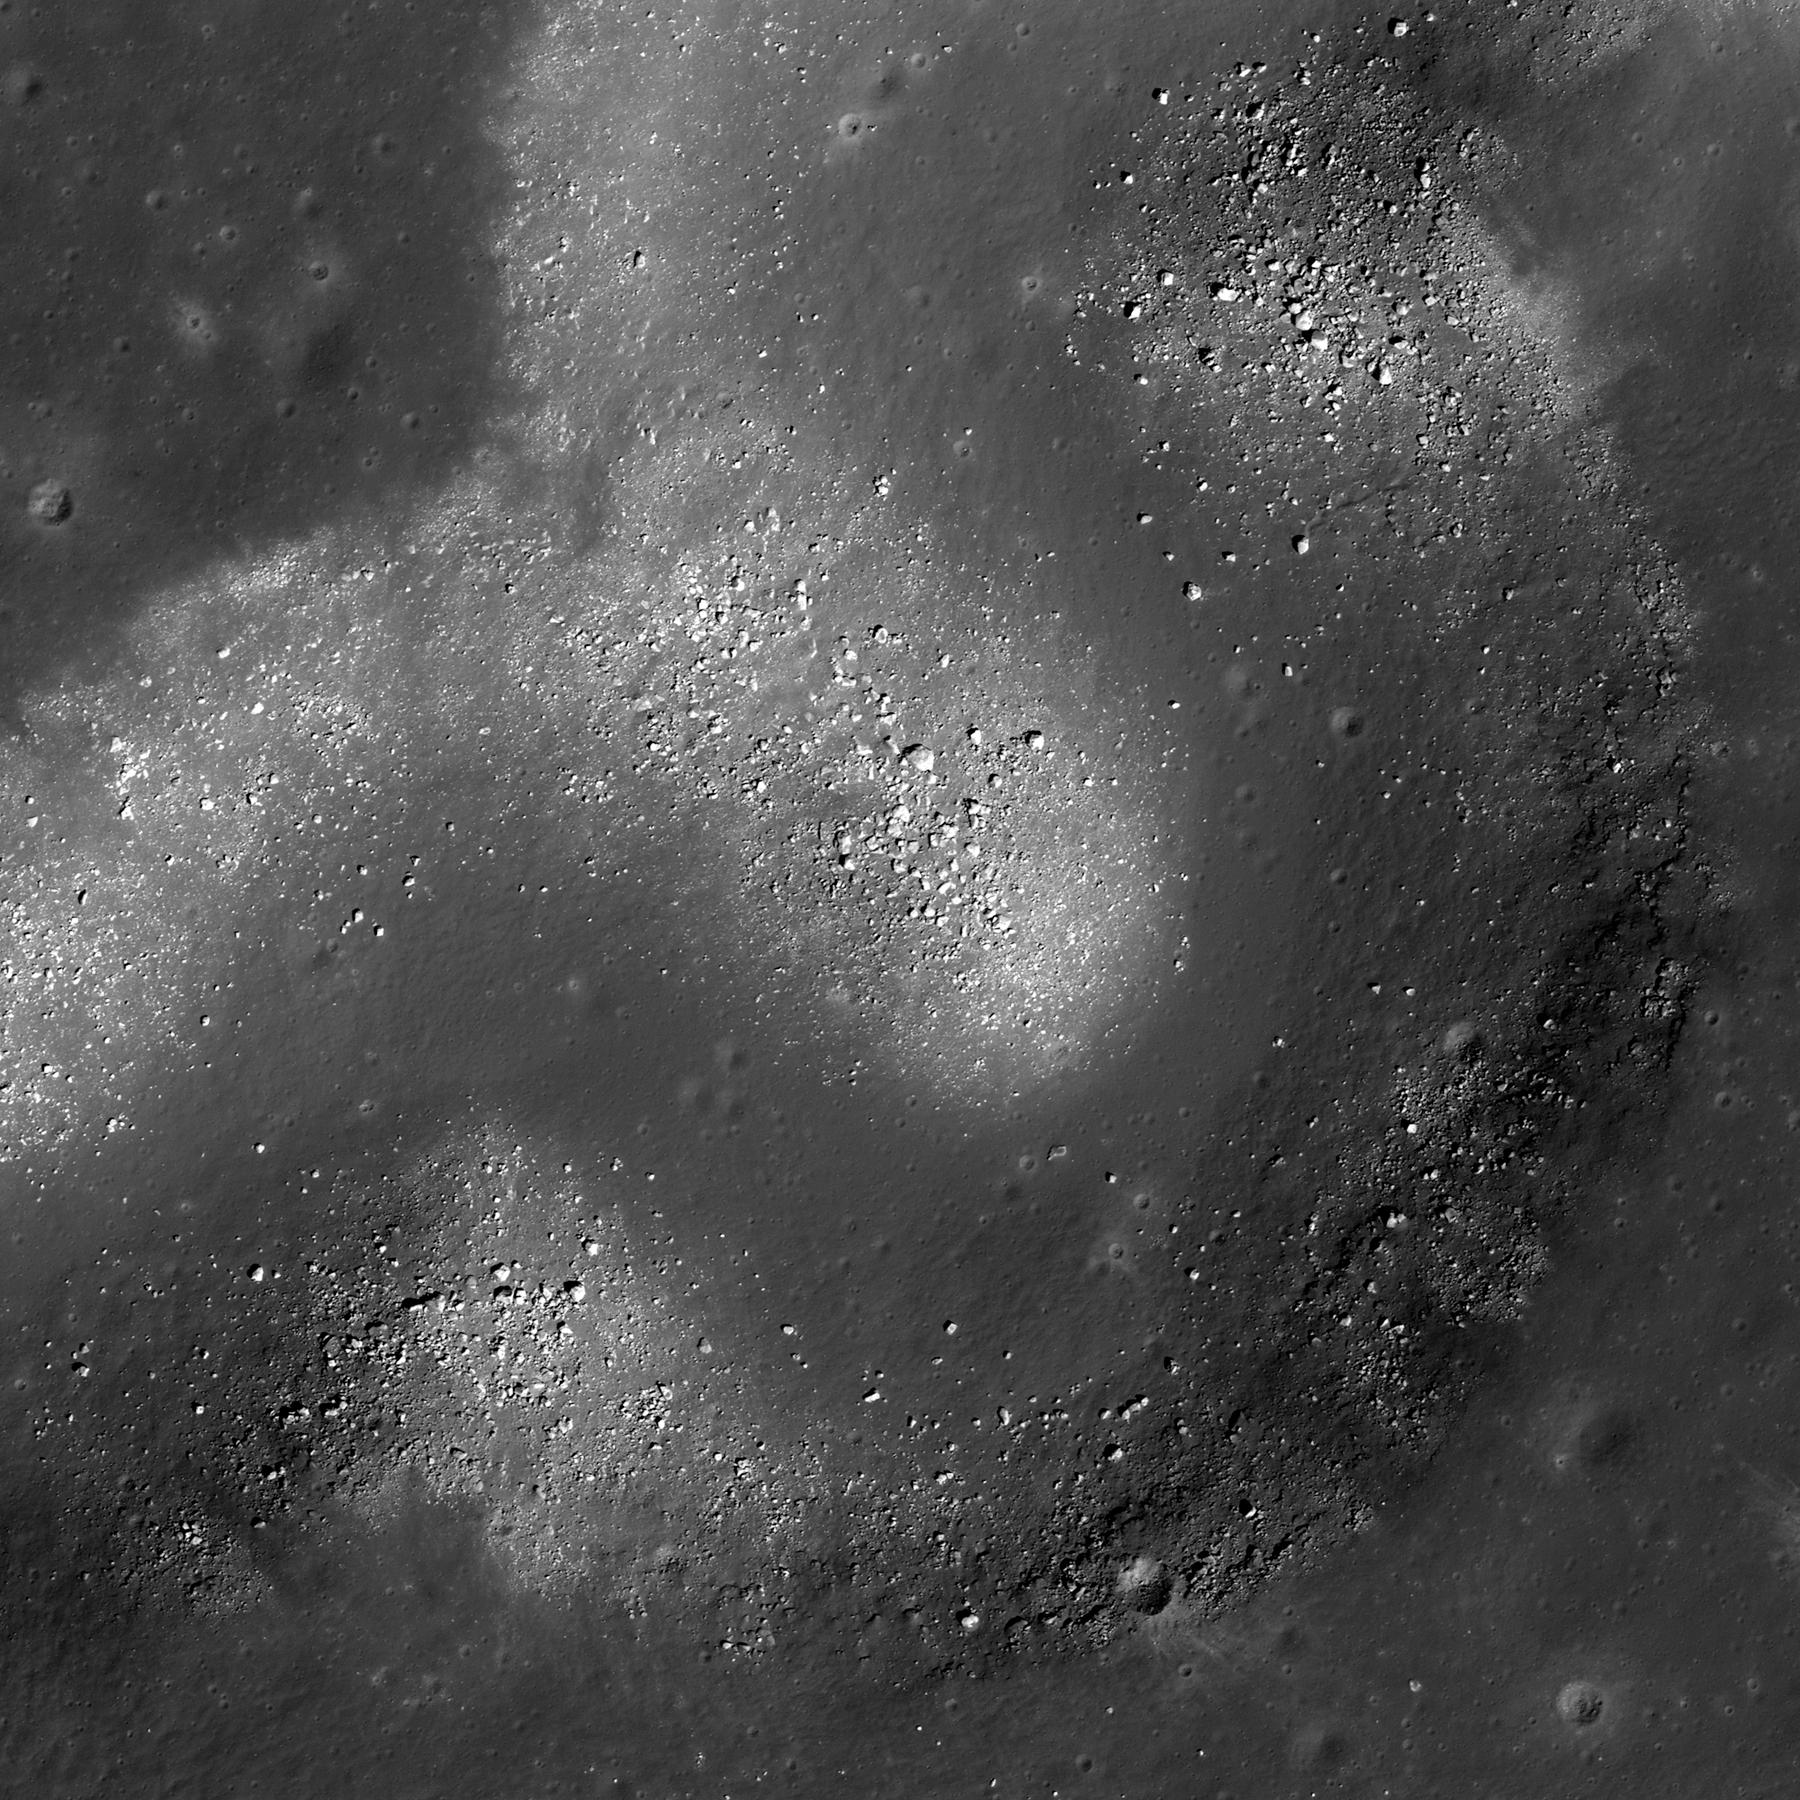
\includegraphics[width=10cm]{nasa.jpg}
		\caption{Image utilisée pour les tests d'optimisation}
		\label{fig:nasa}
	\end{figure}
	
	\subsection{Inverse de la dct}\label{idct}
	\subsubsection{Constantes calculées dans les boucles}
	Dans la fonction \texttt{idct}, plusieurs calculs de constantes étaient effectués à l'intérieur des boucles, dans la 4\ieme{} boucle, ces calculs étaient donc effectués
	$8^4 = 4096$ fois, par image. Le compilateur doit effectuer quelques optimisations afin d'éviter de recalculer trop souvent, cependant il était tout de même
	inutile d'effectuer autant de fois ces calculs, d'autant plus que ce sont des divisions, l'opération la plus couteuse pour un processeur.

	Afin d'éviter la redondance de calculs, j'ai donc mis la valeur du calcul dans des variables statiques : celui-ci sera effectué au premier lancement de
	\texttt{idct} et sera ensuite conservé jusqu'à la fin du programme.

	Les deux opérations concernées étaient : 
	\begin{itemize}
		\item $\frac{\Pi}{16}$, utilisé dans les calculs de cosinus
			\begin{lstlisting}[language=C,numbers=none, caption=Déclaration d'une variable contenant $\frac{1}{\sqrt{2}}$]
static double invSqrt2 = 1 / sqrt(2);
\end{lstlisting}
		\item $\frac{1}{\sqrt{2}}$, utilisé dans la macro \texttt{\bsc{coeffs}}
			\begin{lstlisting}[language=C,numbers=none, caption=Déclaration d'une variable contenant $\frac{\Pi}{16}$]
static double piDivideBy16 = M_PI / 8;
\end{lstlisting}
	\end{itemize}
	\subsubsection{Cosinus}
	Le principal problème de \texttt{idct} était le calcul des cosinus. En effet, un cosinus est un calcul lourd à effectuer, or celui-ci à l'instar des calculs
	de $\frac{\Pi}{8}$ ou de $\frac{1}{\sqrt{2}}$, était placé à l'intérieur des boucles. Ainsi un très grand nombre de calcul étaient effectués.

	Sauf qu'en regardant plus en détail, ces cosinus étaient effectués en fonction des variables $x$, $u$, $y$ et $v$ : variables ne dépendant nullement des
	paramètres de la fonction. Le processeur effectuait donc toujours les même calculs à chaque appel de \texttt{idct}.

	La solution que j'ai trouvé est qu'au premier lancement de \texttt{idct}, je stock les cosinus qui seront nécessaires quel que soit l'appel de \texttt{idct},
	dans le cas ou on aurait plusieurs calculs identiques pour un seul appel, j'ai appliqué un système de \texttt{Hash}.

	Les résultats des cosinus vont être stockés dans un tableau de \texttt{float}, l'indice du tableau sera le paramètre fourni à \texttt{cos}, c'est-à-dire une
	des deux valeurs suivantes : 
	\begin{itemize}
		\item \texttt{(2*y+1)*v}
		\item \texttt{(2*x+1)*u}
	\end{itemize}

	Le résultat d'un cosinus est donc obtenu de la manière suivante :
	\begin{lstlisting}[language=C,numbers=none, caption=Obtention du résultat d'un cosinus]
allCos[(2*y+1)*v];
allCos[(2*x+1)*u];
\end{lstlisting}

Une dernière modification en rapport avec le cosinus à été de remonter la récupération de \texttt{allCos[(2*y+1)*v]} d'une boucle : 
en effet, cette instruction ne dépend que de y et v, il est inutile de la mettre dans la boucle u.
\begin{remarque}
	Cette modification n'a cependant pas fait gagné de temps de calculs, étant donné que ce n'était qu'une lecture RAM très rapide à faire.	
\end{remarque}
	\subsubsection{Déclarations dans les boucles}
	La dernière modification effectuée pour \texttt{idct} était mineure : déplacer les déclarations en dehors de la boucle. En effet, il me paraissait inutile
	d'effectuer une déclaration au début de la boucle, et de détruire la variable à la fin, et ceci $4096$ fois. Cependant, en me renseignant, j'ai découvert que
	le compilateur \texttt{gcc} optimisait cela en se rendant compte qu'il était inutile de libérer la variable : aucun temps n'a donc été gagné grâce à cette
	étape car \texttt{gcc} faisait déjà le travail. 

	Cependant, il est tout de même plus propre de ne pas se reposer sur le compilateur et d'effectuer nous même les optimisations, en effet, se reposer sur le
	compilateur peut être dangereux en fonction des versions du compilateur. Quant est-t-il de Mingw, Cygwin, Visual C++, \ldots ?
	\subsection{Parallélisme avec \texttt{openmp}}
	La parallélisation permet d'utiliser plusieurs cœurs simultanément, ce qui pourrait hypothétiquement accélérer le calcul sur les matrices. En effet certaines
	boucles pourraient être faites par plusieurs threads.

	Cependant, en pratique, cette optimisation est inutile pour notre problème. En effet, le temps qui pourrait être gagné par le traitement paralléliser est
	perdu à cause de la communication entre threads et de leur gestion : sur un petit volume de données, cela est donc contre-productif.

	Or, notre projet comporte des calculs qui s'effectuent principalement sur des blocs de $8 \times 8$ : ce sont donc des petites itérations, bien que
	nombreuses. \\
	L'utilisation de OpenMP serait donc plus intéressantes pour des boucles parcourant de gros volumes de données.

	Les boucles les plus intéressantes à paralléliser sont celles qui peuvent s'effectuer en parallèle indépendamment de l'itération courante, ce sont donc les
	boucles concernant la vectorisation du côtés de la compression et la << dévectorisation >> du côtés de la compression.
	\subsection{Gain de temps grâce à l'optimisation}\label{statsOpti}
	La figure \ref{fig:statsOpti} montre les différents gains de performances effectués tout au long de l'optimisation. 
	\begin{description}
		\item[Aucune] Aucune optimisation
		\item[Nombre de boucles] Optimisation de mon code afin de diminuer au maximum le nombre de boucles
		\item[\texttt{idct}] Optimisation de la fonction \texttt{idct} comme détaillé section \ref{idct}
		\item[OpenMP] Utilisation de la bibliothèque OpenMP afin de paralléliser le travail
	\end{description}
	\begin{figure}[H]
		\centering
	\begin{tikzpicture}[scale=.7]
		\begin{axis}[xtick={1,20,40,60},xlabel={\textbf{Type d'optimisation}}, ylabel={\textbf{Tempx d'éxecution (s)}}, xticklabels={Aucune, Nombre de boucles, \texttt{idct}, OpenMP}, legend entries={Compression, Decompression}, width=13cm]
			\addplot coordinates{(1,0.410)(20,0.207)(40,0.200)(60,0.130)};
			\addplot coordinates{(1,10.732)(20,10.536)(40,0.497)(60,0.310)};
		\end{axis}
	\end{tikzpicture}
	\caption{Statistiques sur le temps gagné grâce aux optimisations}
	\label{fig:statsOpti}
\end{figure}
Nous pouvons donc observer qu'au vu de sa rapidité, la compression n'était pas optimisable : il parait extrêmement difficile de gagner ne serait-ce que 30ms,
notamment grâce à la fonction \text{dct} qui effectue la majorité de ses calculs directement en binaire. 

Cependant, grâce à notre optimisation, nous avons pu avoir une décompression $\frac{10.510}{0.502} = 21$ fois plus rapide ! 

\hspace{-50px}
\begin{tabular}{cc}
\begin{minipage}{0.5\textwidth}
	\begin{lstlisting}[language=Bash,linewidth=280px, caption=Sans optimisation]
 (ssh) aroquemaurel@aokiji <noOptimize>
 [0] % time ./compressor 0 nasa.xxx nasa.pgm

./compressor 0 nasa.xxx nasa.pgm  10,47s user 0,02s system 99% cpu 10,510 total
 \end{lstlisting}
\end{minipage}
&
\begin{minipage}{0.5\textwidth}
	\begin{lstlisting}[language=Bash,linewidth=280px, caption=Avec optimisations]
(ssh) aroquemaurel@aokiji <master>
[0] % time ./compressor 0 nasa.xxx nasa.pgm 

 ./compressor 0 nasa.xxx  nasa.pgm 0,48s user 0,01s system 99% cpu 0,502 total
 \end{lstlisting}
\end{minipage}
\end{tabular}

	\appendix
	\listoffigures
	\lstlistoflistings

\end{document}
